%-----<<< APPENDIXS >>>-----
\cleardoublepage
\def\appendixname{Appendix}
%\begin{appendices}
\begin{appendix}
\captionsetup{list=no}
\updatechaptername

\chapter{Mechanical design}
\label{a:mechanical-design}

Mechanical drawings of our FWMAV are shown in Figures~\ref{fig:assembly_labels_top} --~\ref{fig:rocker}. Pictures of the assembled vehicle are shown in Figures~\ref{fig_photo_side} and~\ref{fig_photo_top}, showing top and side view of the vehicle. Figure~\ref{fig_photo_shaft} shows the sealed and marked shaft, which was a necessary measure to prevent the shaft from slipping under higher loads (such as during change from $\delta$ to $-\delta$). Figure~\ref{fig_photo_start_pos} shows the correct initial position of the wings that is necessary because there is no absolute position sensor of the motor angle. The user has to place the wings into the initial position at the beginning of each experiment.

The first iteration of the vehicle was built at Wright State University (WSU). The second (modified) version was build at Portland State University (PSU). The motors and the wing assembly is identical for both versions, and could be further improved. The second version contains smaller control electronics (this was achieved by tightly packaging the electronic components), a smaller and lighter battery, and a smaller flotation device made from a lighter foam. All components in the second version are more tightly packaged, resulting in a more compact and more nimble vehicle.

Properties of both versions are compared in Table~\ref{tab-vehicle-characteristics}. The second version is lighter and more agile. It can follow the trajectory faster than the first version. The custom PCB boards for power distribution and control could be further improved in future iterations.

Both versions are using two brushless DC motors Faulhaber series 1028\_B, product code 1028S006BIEM3-1024. The motor is 10~mm in diameter, 6.0~V coil and 1.2~mm diameter output shaft. The mechanical drawing of the motor is shown in Figure~\ref{fig_drawing_motor}. The motor assembly includes series IEM3, integrated 3 channel magnetic incremental encoder with 1024 Counts-Per-Revolution (CPR) resolution. The motor uses planetary gearhead 10/1 with 4:1 ratio.

\begin{table}%[ht!]
\centering
\renewcommand{\arraystretch}{1.0}
\begin{tabular}{>{\small}l>{\small}cccc}
\hline
Property & 1st iteration & 2nd iteration & Comments\\
\hline
\rowcolor{Gray}
Weight & 406 g (14.3 oz) & 180 g (6.3 oz) & 55\% decrease\\
Diameter & TBD cm (TBD in) & TBD cm (TBD in) & 30\% decrease\\
\rowcolor{Gray}
Current cons.& $\leq1$A & At max speed of& 40~rad/s (6.2~Hz) \\
Peak cur. cons. & 3~A & Immediately & after start \\
\rowcolor{Gray}
Battery & 2 cell 3Ah & 2 cell 300mAh & 3hrs $\rightarrow$ 20 min flight \\
\hline
\end{tabular}
\newline
\caption[Electrical and Mechanical Characteristics of the vehicle]{Electrical and Mechanical Characteristics of the vehicle, for both 1st and 2nd iteration}
\label{tab-vehicle-characteristics}
\end{table}

\begin{figure}
\centering
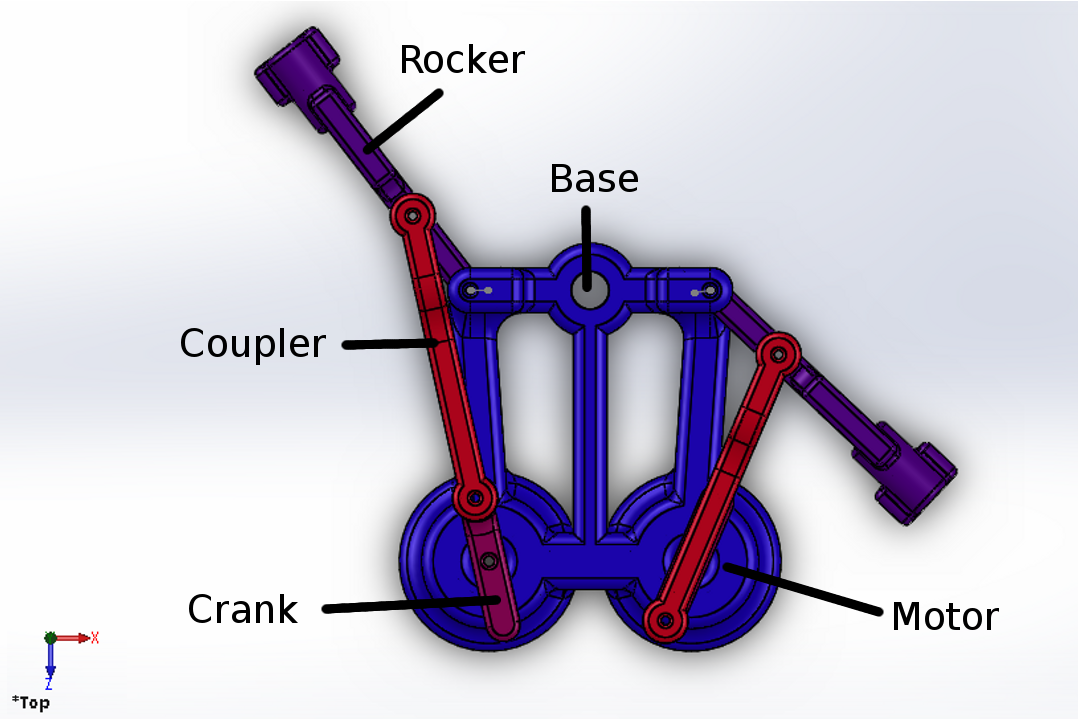
\includegraphics[width=0.8\textwidth]{Files/Figures/cad_assembly_labeled.png}
\caption{Top view of the actuator assembly (actual size)}
\label{fig:assembly_labels_top}
\end{figure}

\begin{figure}
\centering
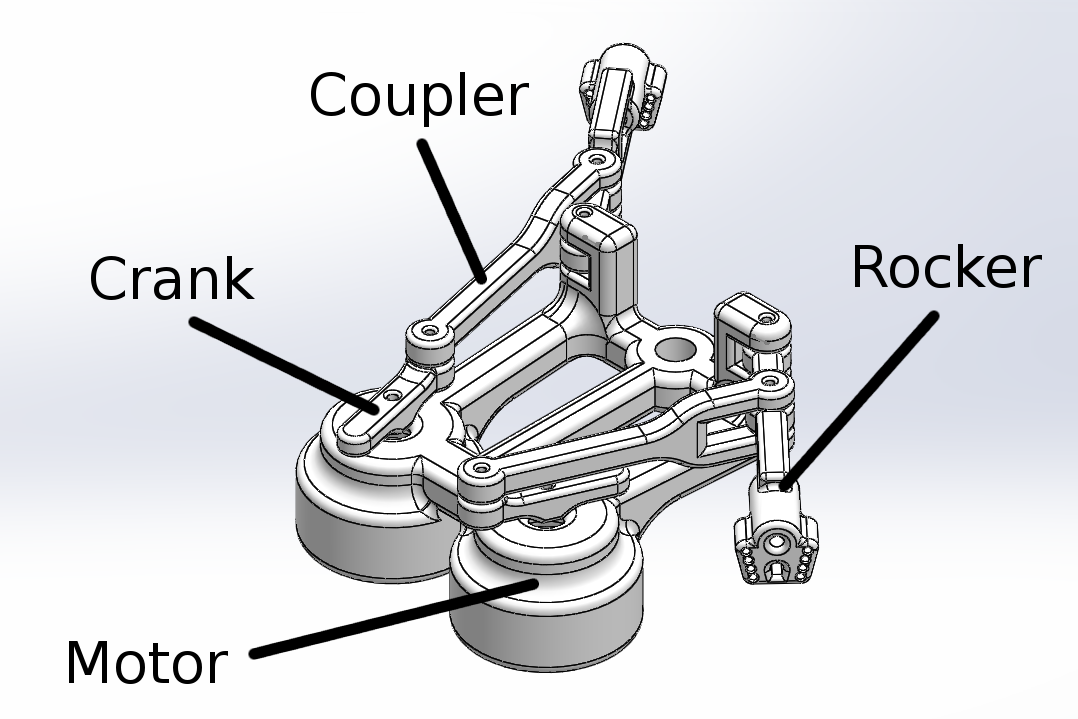
\includegraphics[width=0.8\textwidth]{Files/Figures/cad_assembly_iso.png}
\caption{Isometric view view of the actuator assembly (actual size)}
\label{fig:assembly_labels_iso}
\end{figure}

\begin{figure}
\centering
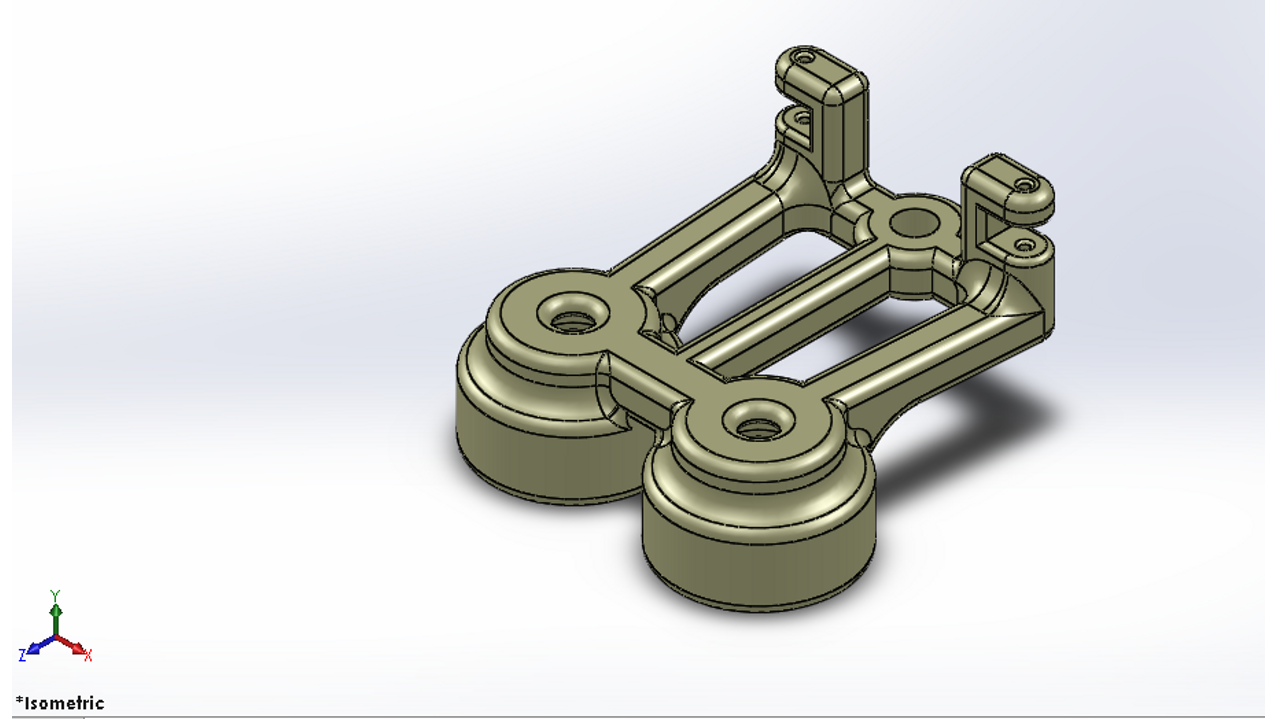
\includegraphics[width=\textwidth]{Files/Figures/base.png}
\caption{A base (isometric view, not to scale)}
\label{fig:base}
\end{figure}

\begin{figure}
\centering
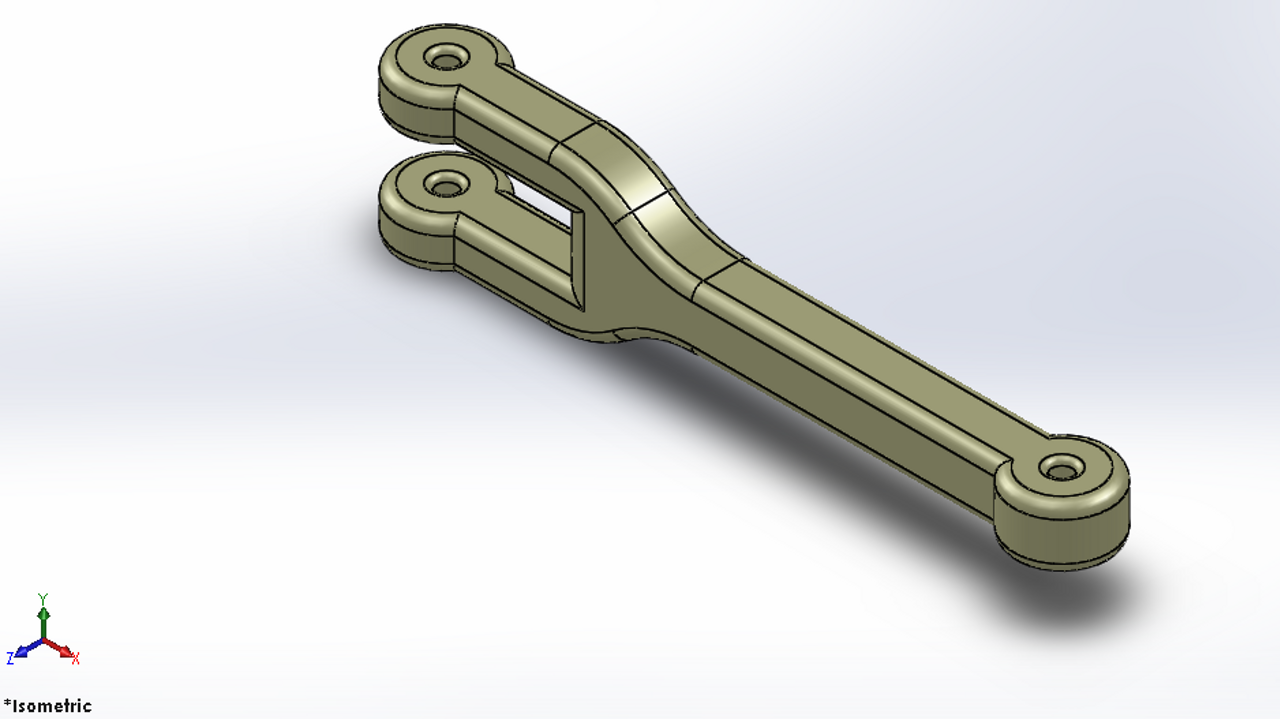
\includegraphics[width=\textwidth]{Files/Figures/coupler.png}
\caption{A coupler (isometric view, not to scale)}
\label{fig:coupler}
\end{figure}

\begin{figure}
\centering
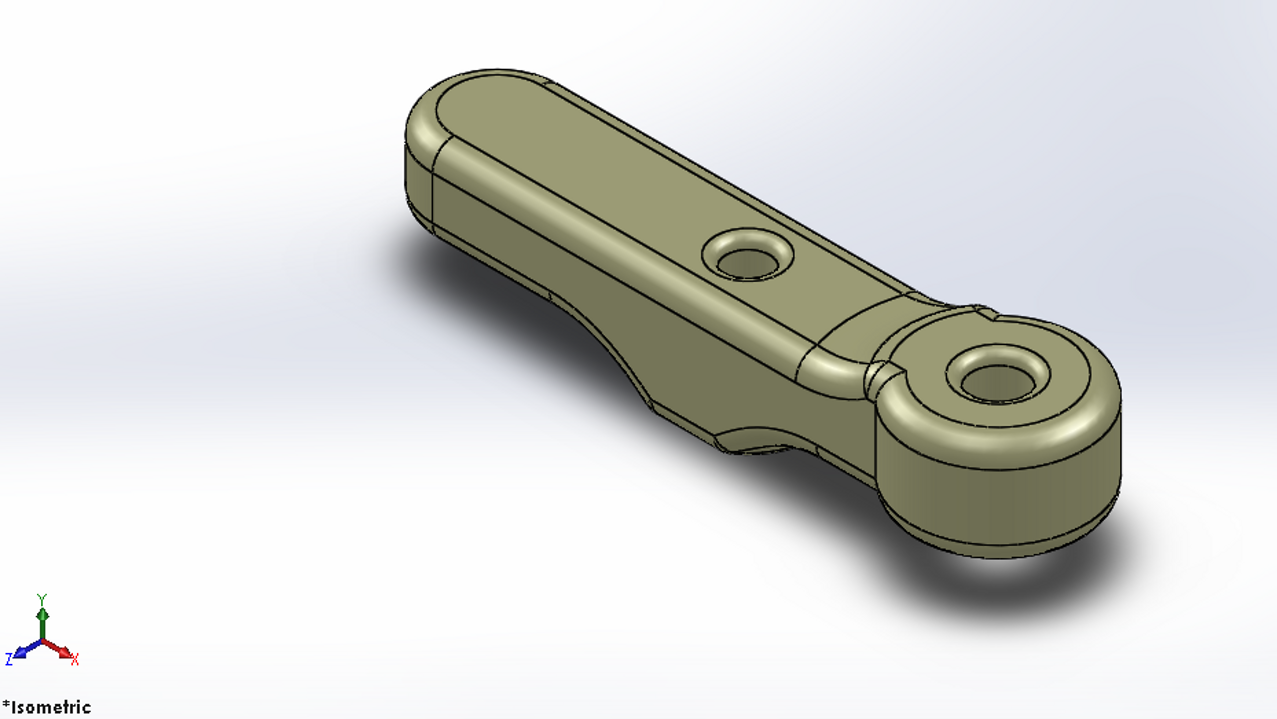
\includegraphics[width=\textwidth]{Files/Figures/crank.png}
\caption{A crank (isometric view, not to scale)}
\label{fig:crank}
\end{figure}

\begin{figure}
\centering
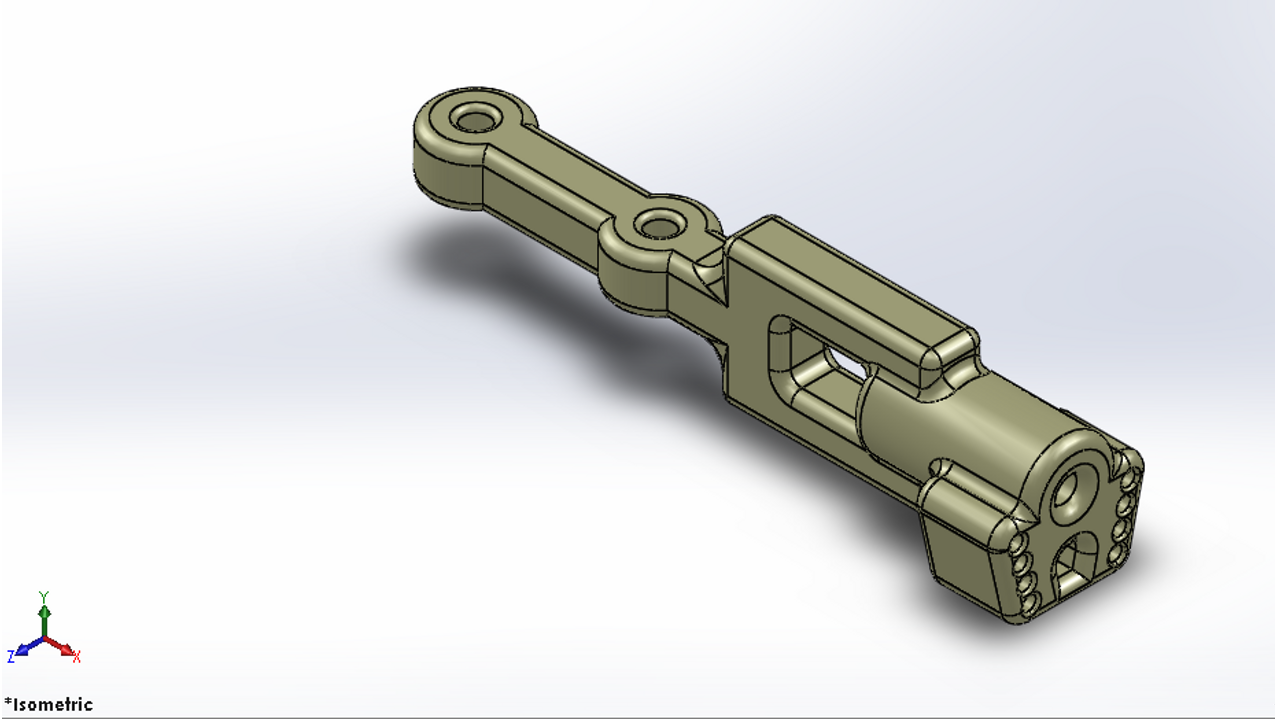
\includegraphics[width=\textwidth]{Files/Figures/rocker.png}
\caption{A rocker (isometric view, not to scale)}
\label{fig:rocker}
\end{figure}

\begin{figure}
\centering
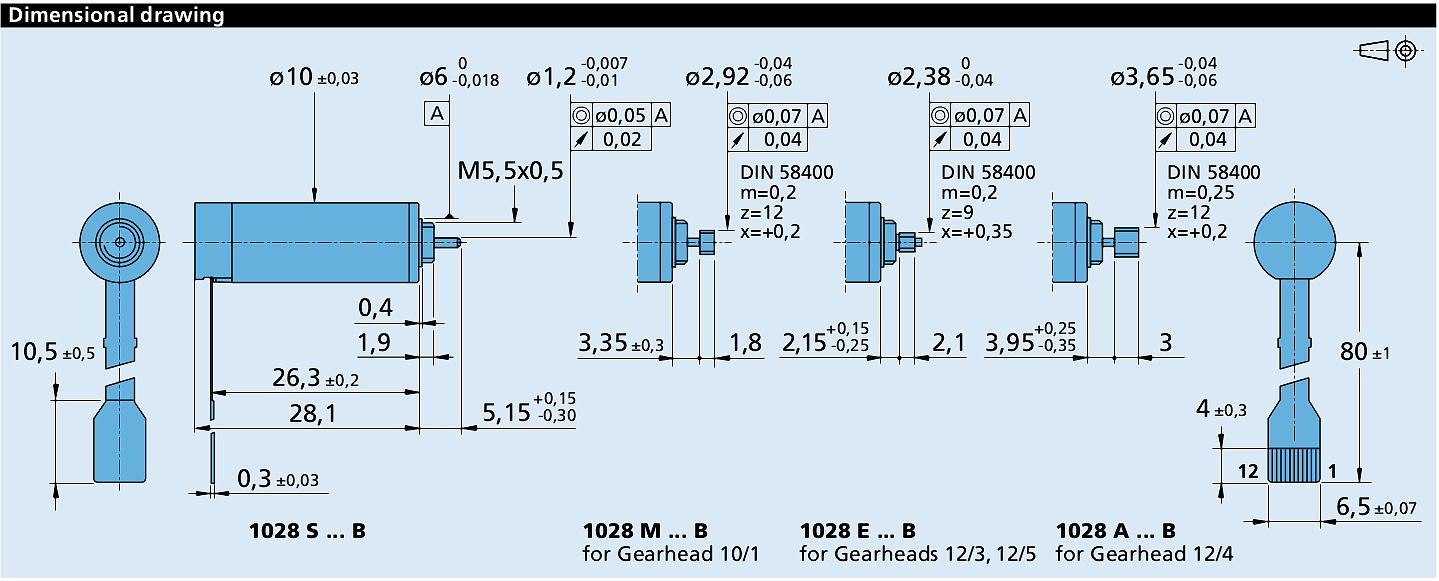
\includegraphics[width=17cm, angle=90]{Files/Figures/motor_drawing.png}
\caption[Faulhaber series 1028B DC motor]{Faulhaber series 1028\_B brushless DC motor, product code 1028S006BIEM3-1024; The motor can be ordered at \url{http://www.micromo.com/1028s006biem3-1024.html}}
\label{fig_drawing_motor}
\end{figure}

\begin{figure}
\centering
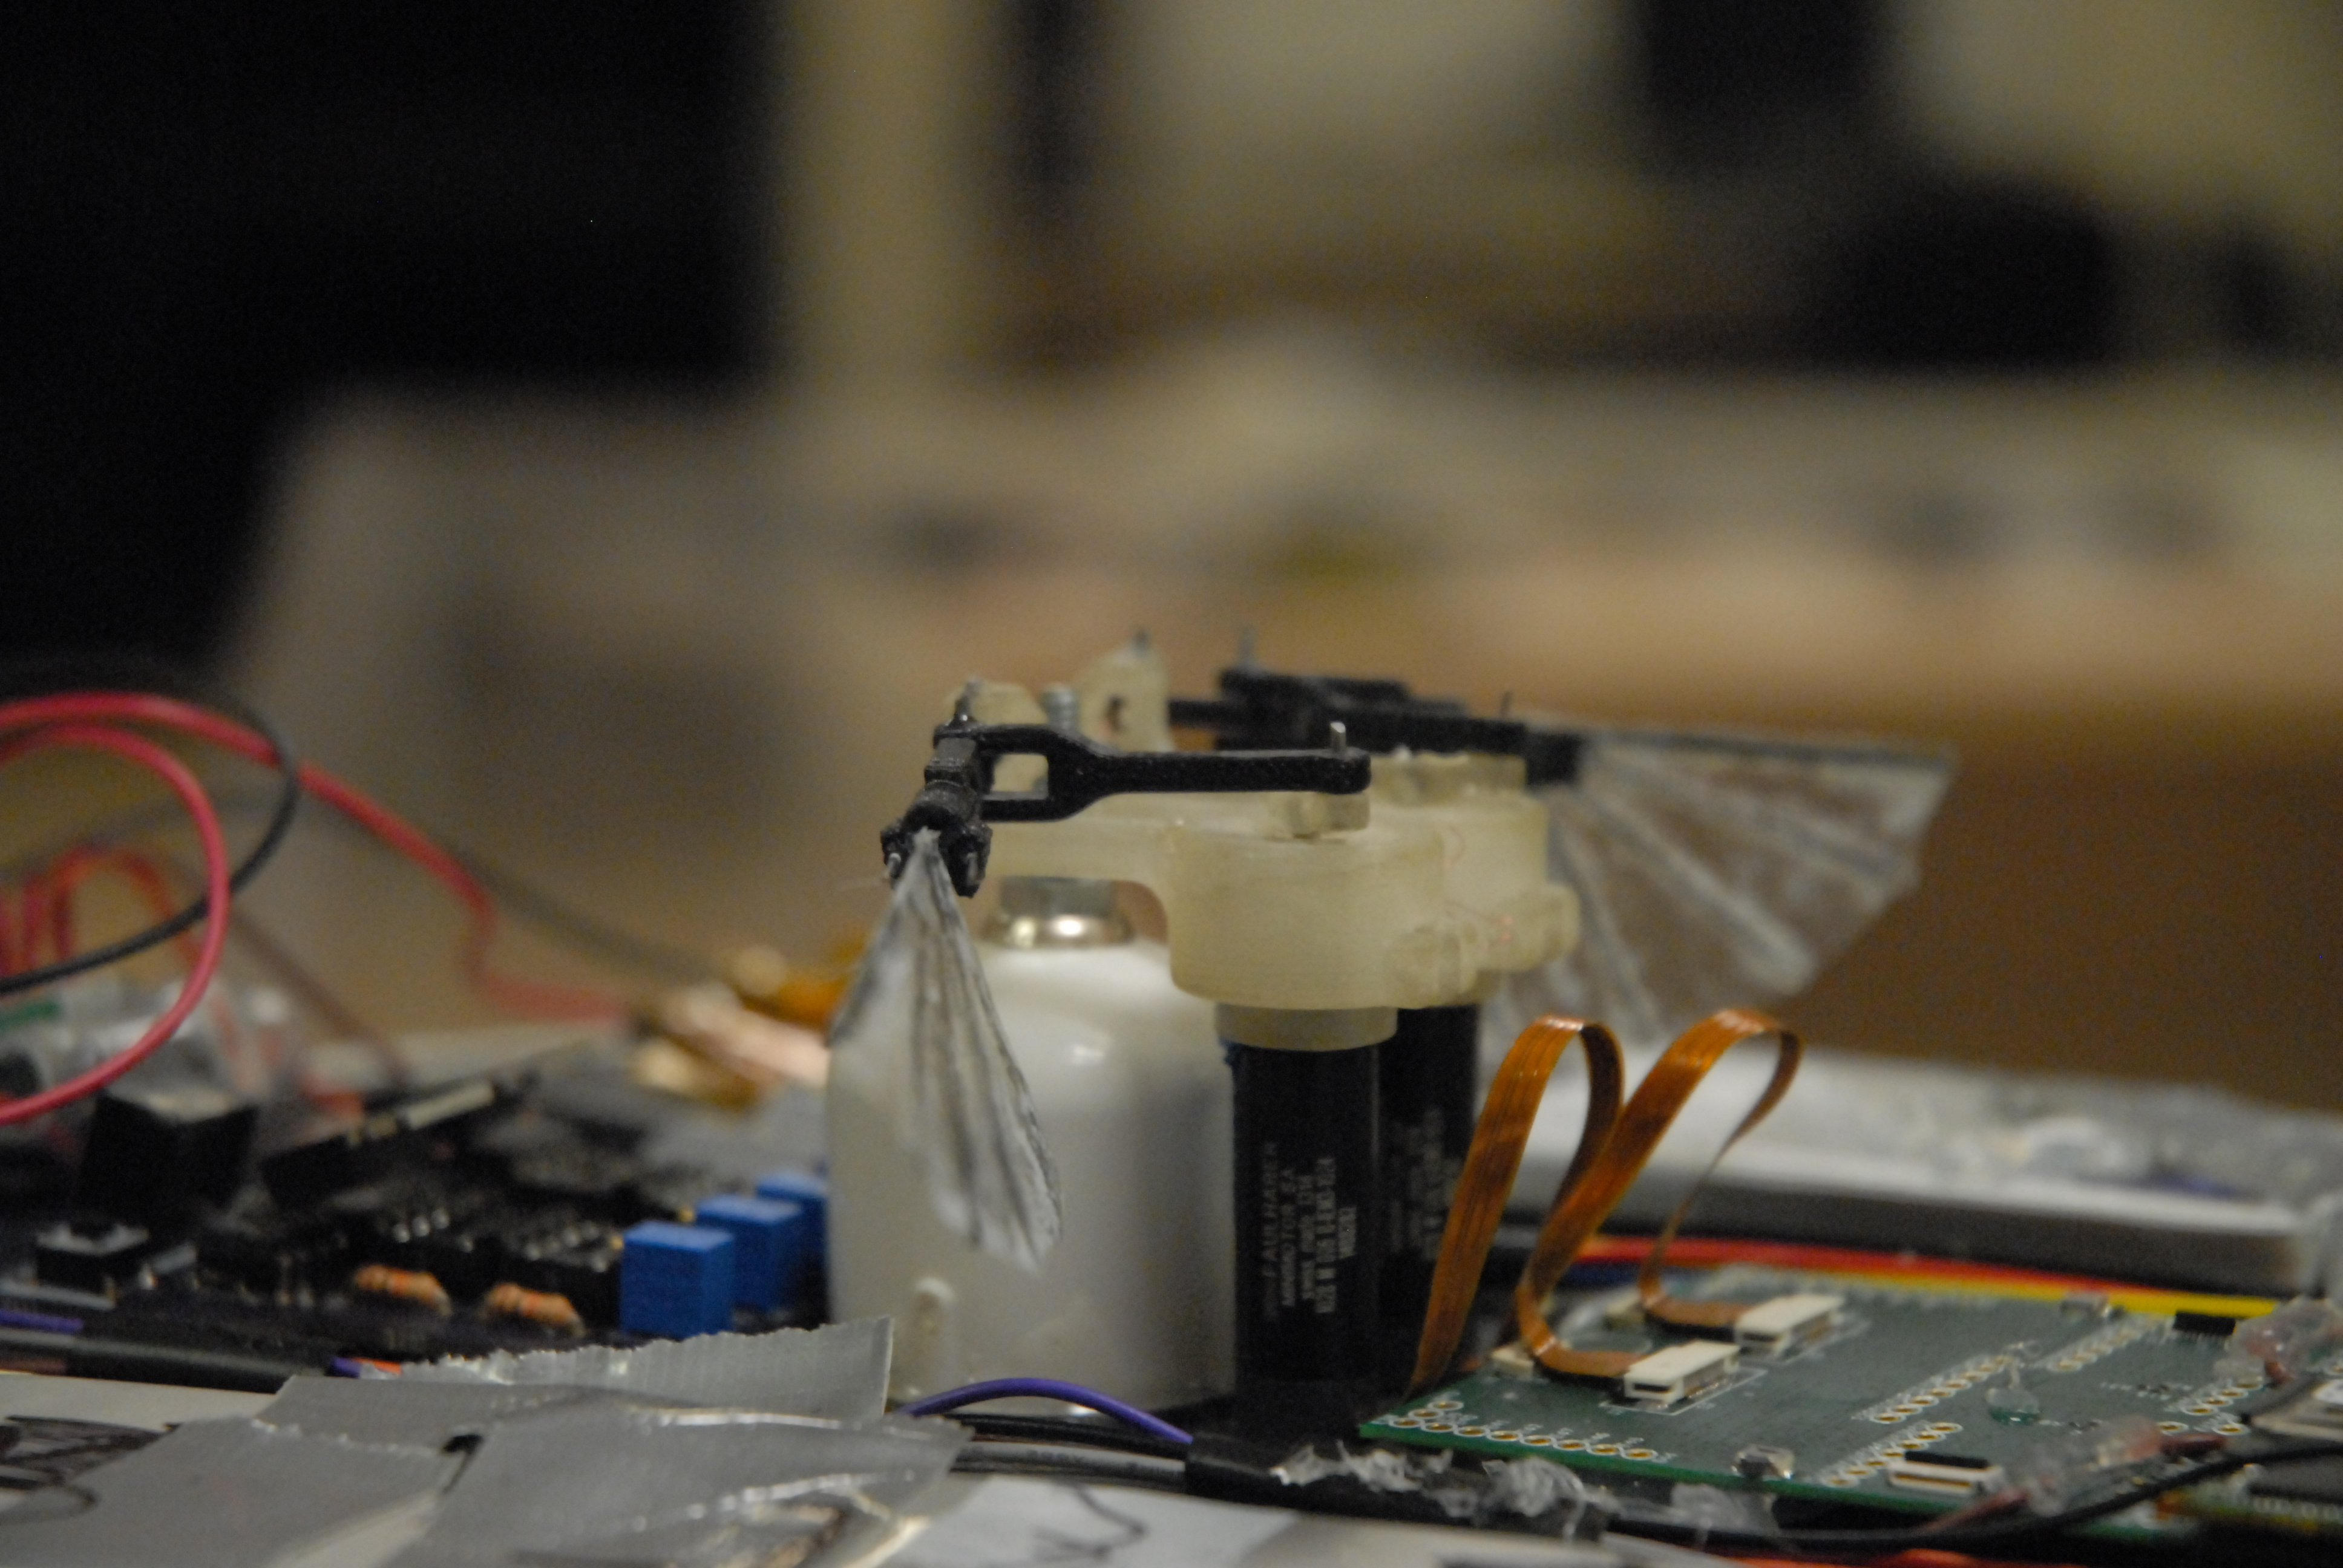
\includegraphics[width=12.5cm]{Files/Figures/photo_side.jpg}
\caption{Side view.}
\label{fig_photo_side}
\end{figure}

\begin{figure}
\centering
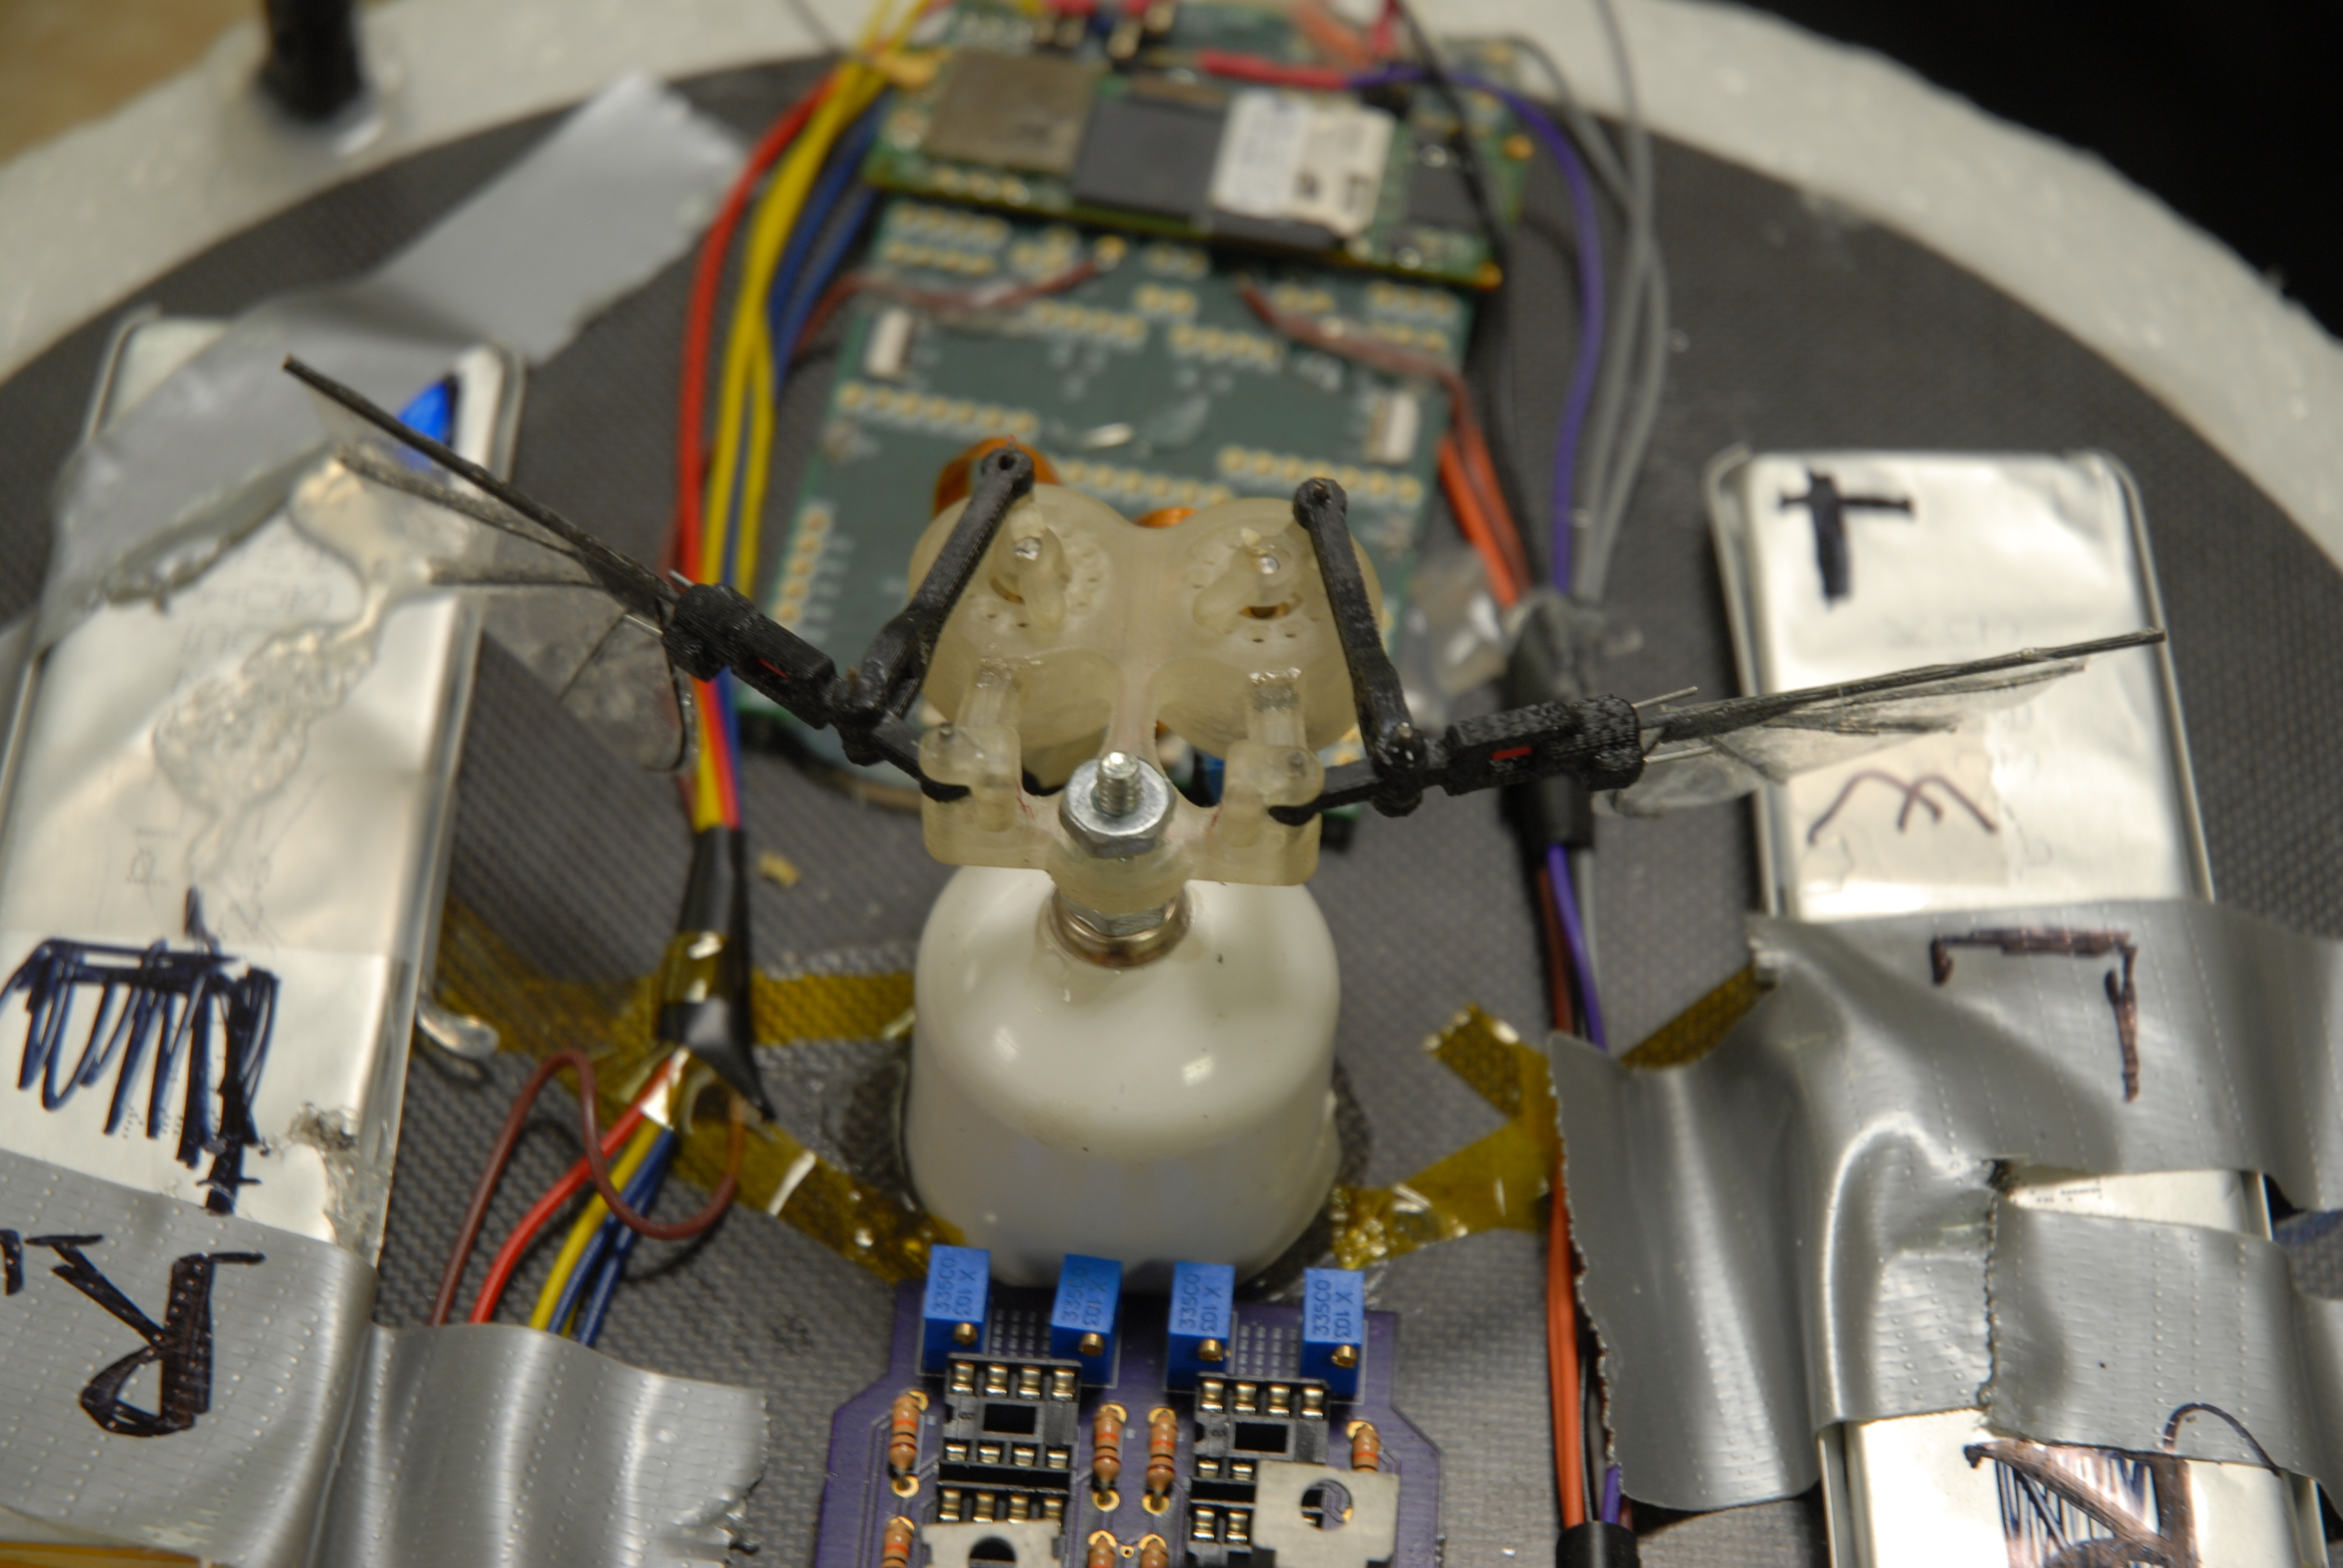
\includegraphics[width=12.5cm]{Files/Figures/photo_top.jpg}
\caption{Top view.}
\label{fig_photo_top}
\end{figure}

\begin{figure}
\centering
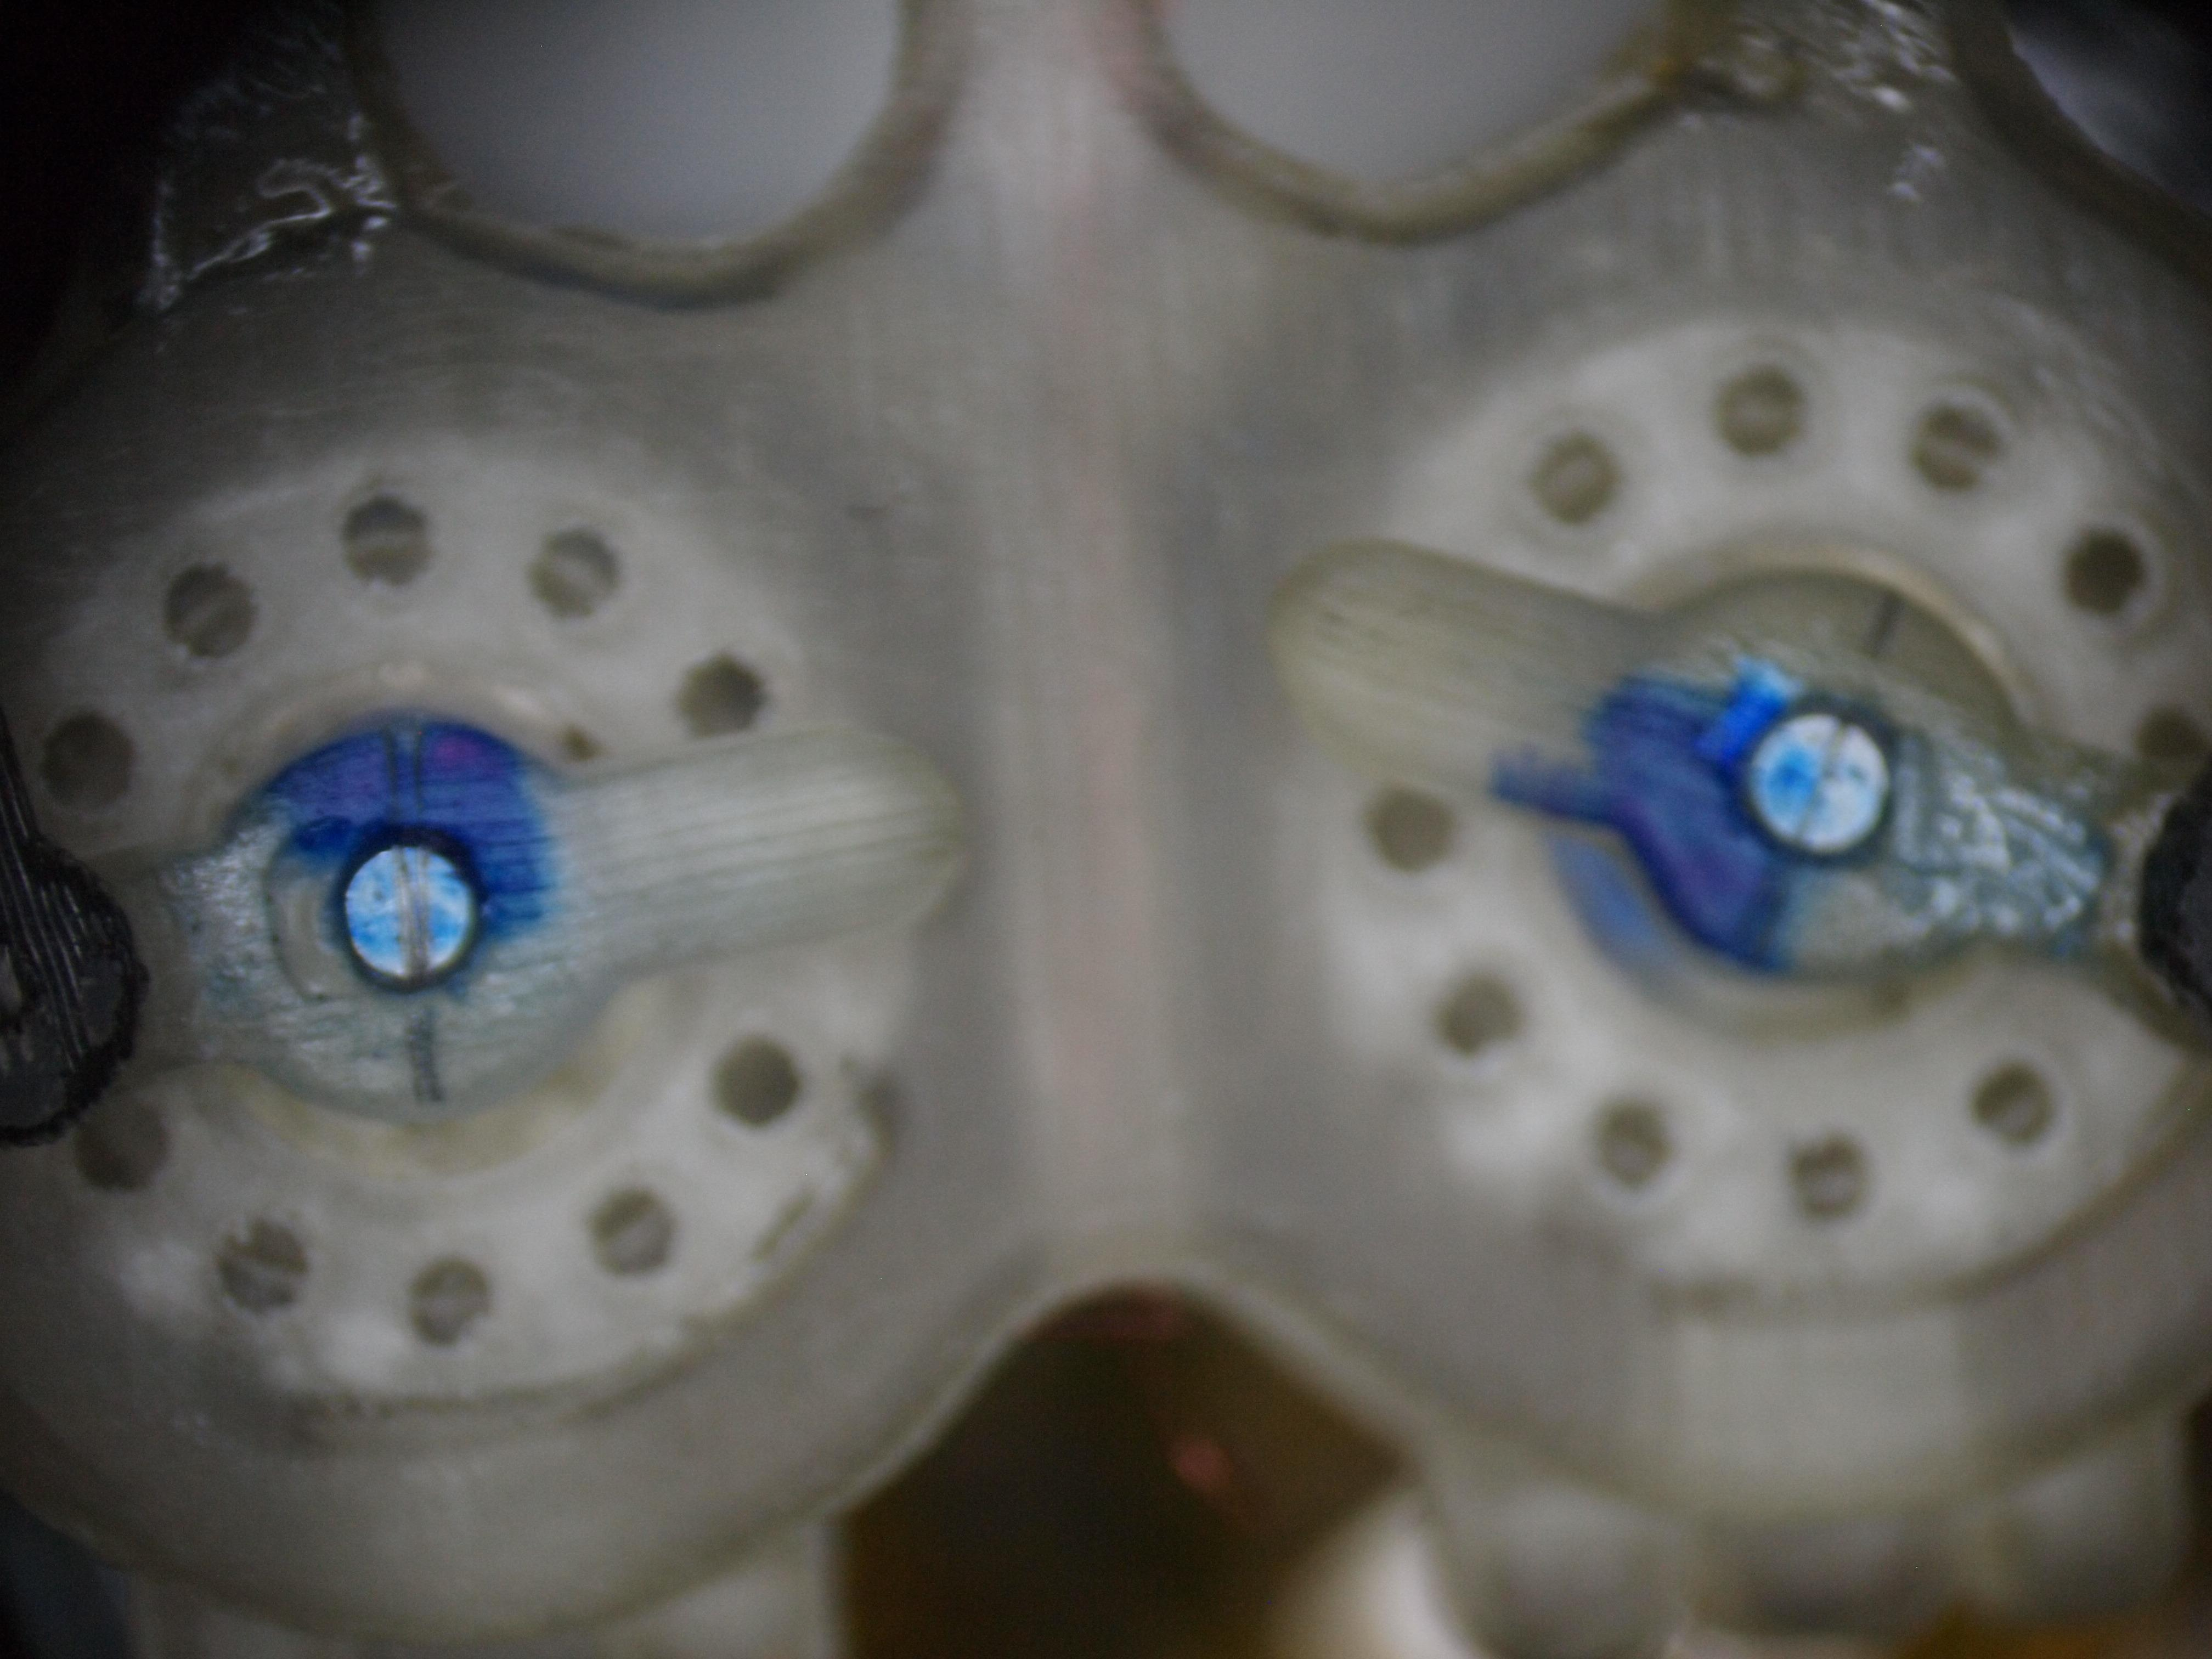
\includegraphics[width=11cm]{Files/Figures/sealed_shaft.jpg}	
\caption[Sealed shaft]{Sealed shaft with markers to prevent shaft slippage}
\label{fig_photo_shaft}
\end{figure}

\begin{figure}
\centering
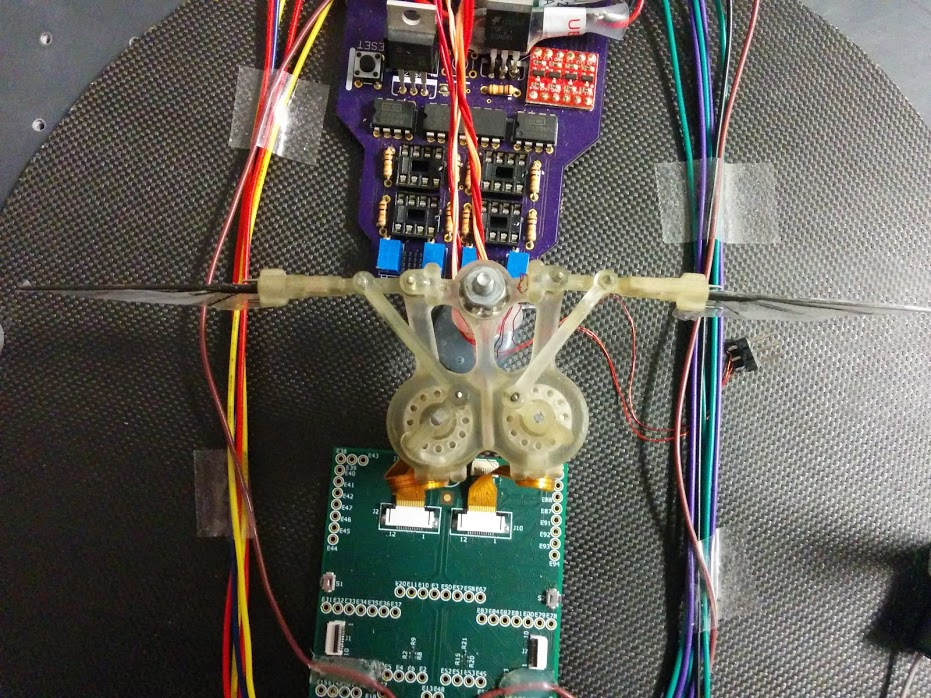
\includegraphics[width=11cm]{Files/Figures/start_pos.jpg}
\caption{Starting position of the wings}
\label{fig_photo_start_pos}
\end{figure}


\chapter{Software Architecture}
\label{a:code}
The code is split into four main layers. Currently different programs contain separate layers, but in the future all layers can be used in one embedded program while keeping the functionality. The code has these layers:
\begin{enumerate}
\item Motor firmware -- directly controls the motors by driving FET transistors
\item Multi Agent System -- controls the vehicle (see Section~\ref{ch:approach}
\item Pose estimation System -- captures raw image from a video camera and applies clever image processing algorithms on it to find out the vehicle's pose (see Section~\ref{sec-environment})
\item Graphical User Interface (GUI) -- to let user command (start, stop, restart) the vehicle and to show telemetry from the vehicle
\end{enumerate}

Each layer is further described below.

\section{Motor Firmware}
\label{a-firmware}
This is the low level code that directly gives commands to the motors and reads the outputs of the encoders. This code runs on PIC micro controllers (MCU) -- two PICs for each motor -- and typically the user don't interact with it. The firmware was developed and is maintained by Hermanus Botha\footnote{wkjid10t@gmail.com}.

\section{Multi Agent System}
\label{a-mas}
Is the implemented MAS from Chapter~\ref{ch:approach}. It determines desired control inputs $\delta$ and $\omega$ based on the state of the vehicle and its pose. It uses two sub-layers: \textit{Application Programming Interface (API)} to connect with the motor firmware and \textit{UDP communication} to connect with the Pose Estimation System.

\subsection{API}
\label{subsec-api}
The API is running on the embedded Linux on Gumstix Overo, and is setting wing beating frequency and delta values. API gives commands to the PICs over SPI, the PICs then translate these commands into signals for the motors. The API, developed by Hermanus Botha, consists of several functions that can be called from user application. The most important ones are:
\begin{itemize}
\item \textit{set\_frequency()}, \textit{set\_delta()} which sets $\omega, \delta$ for corresponding wings
\item \textit{init()} initializes the motors before they can be used
\item \textit{close()} closes the communication with motors in an orderly manner
\end{itemize}

\subsection{UDP Communication}
The highest layer of communication takes place over WiFi network, and can be fully defined by the user. It requires a server (typically running on a laptop), and a client program (running on the robot). The server waits for an incoming connection from a client, and once it is established it keeps communication with the client alive. The clients tries to connect with the server, and if successful it initializes the wings and waits for commands from the server. In the most basic example there are two UDP packets:
\begin{itemize}
\item Server $\rightarrow$ Client: four float numbers with desired values of $\delta_L, \delta_R, \omega_L, \omega_R$ in rad/s
\item Client $\rightarrow$ Server: four float numbers with actual\footnote{i.e. the values that API gets from PICs} values of $\delta_L, \delta_R, \omega_L, \omega_R$ in rad/s
\end{itemize}

The desired values of $\delta, \omega$ can be passed to the server either from a user application running on the same machine (typically a laptop), or directly from the user - for example from the console. 


\section{Pose Estimation System}
This system is written in C++ and uses OpenCV library for image processing. The algorithm is in detail described in Section~\ref{sec-environment}. Although developed separately (mostly for the ease of testing), it is now integrated into the GUI. That way the user can easily control the pose estimation system (for example start/stop recording the video), and the whole program is more compact (no need to pass data between two separate processes).

\section{Graphical User Interface}
Currently we have two user programs that can communicate with the vehicle. One is a sample server with console, so the user can set the $\delta, \omega$ values manually by typing commands. The other program is build using \href{http://www.qt.io/}{Qt framework}, and allows the user to set the desired values using sliders (in the manual mode), or to control the MAS and the pose estimation system (in the autonomous mode).. This Qt application also reads data from the camera, localizes the vehicle in the watertank and will run the basic evolution algorithms to determine the basic movements. The GUI is shown in Figure~\ref{fig-gui}.

\begin{figure}
\centering
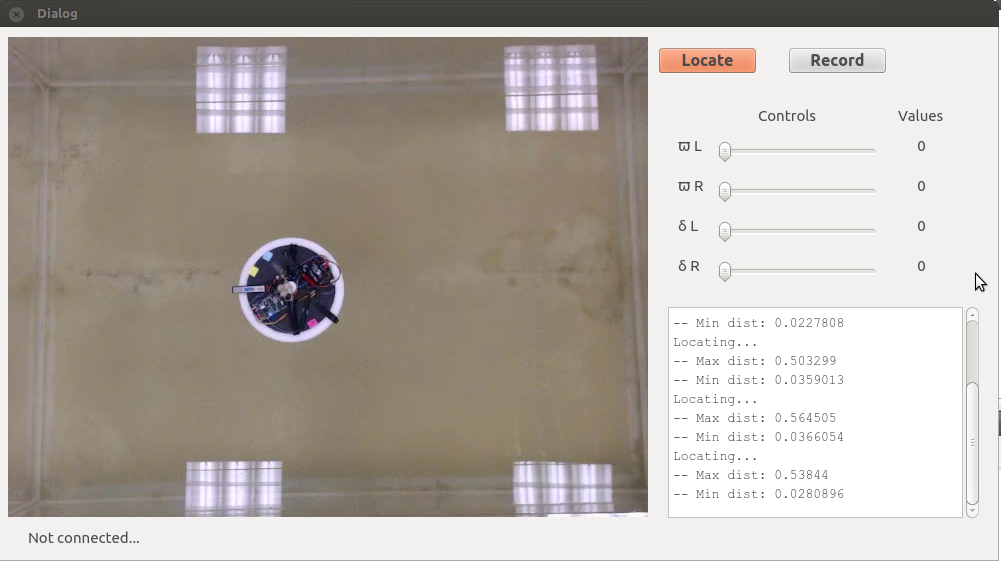
\includegraphics[width=13.5cm]{Files/Figures/gui.png}
\caption[Qt GUI with camera feed]{Qt GUI with camera feed on the left, user controls in the top right and console on the bottom right.}
\label{fig-gui}
\end{figure}

\section{Application Notes}
% Why not Matlab etc
One might ask why we are not using Matlab, since it makes developing learning algorithms very simple. The main problem is that server example is running in Linux (Ubuntu 12.04) and Matlab available at the university doesn't support using webcams in Linux \footnote{\url{http://unix.stackexchange.com/questions/\\87001/connection-error-for-linux\\-webcam-driver-for-matlab}}. We are using Qt GUI.


\newpage

\subsection{Initialization procedure}
The procedure to initialize the vehicle needs to be done before the experiments can be conducted, and goes as follows:

\begin{enumerate}
\item Turn on the WiFi router
\item Connect laptop to WiFi
\item Turn on the vehicle
\item Establish SSH connection
\item Loop through:
	\begin{enumerate}
	\item Reset PICs using reset switch (vehicle)
	\item Align wings to their apexes (vehicle)
	\item Start the server (laptop)
	\item Start the client (vehicle)
	\item Wait for initialization (vehicle)
	\item Send commands (laptop)
	\item When done close the server
	\end{enumerate}
\item Disconnect everything
\end{enumerate}

Steps 1 -- 4 are needed only once per session, steps 5 -- 6 have to be done before each new measurement.


\chapter{Additional resources}
\label{c:additional-resorces}

\begin{center}
Additional resources (such as source code, recoreded data and video) are available at \url{http://podhrmic.github.io/}
\end{center}

\end{appendix}

